\chapter{Verwandte Arbeiten}
Die Idee für interaktive Türschilder wurde schon in verschiedenen wissenschaftlichen Ausarbeitungen sowie in der Praxis aufgefasst.
Die Gruppe um Keith Cheverest et al. von der Universität Lancaster hat mehrere Paper für ihr Türschild-System ``Hermes''\cite{cheverest:2003:paper} bereits ab 2003 veröffentlicht.
Das Projekt ``NetBoards'' von Errol Wood\cite{wood:2014} von der Universität Cambridge behandelt eine aktuellere Version interaktiver Türschilder.
% Andere Projekte Einleitung
\todo

\section{Hermes}
Das Hermes System\cite{cheverest:2003:paper}\cite{cheverest:2003:article}\cite{cheveres:2005:hermes-bluetooth} ist eines der ersten Versionen interaktiver digitaler Türschilder im Bürobereich.
Es diente dazu herauszufinden, ob die \textquote{traditionelle Methode Nachrichten in einem halbwegs öffentlichem Raum (wie beispielsweise vor Büros in einem Forschungsinstitut) mittels Post-It Zetteln zu hinterlassen durch eine digitale Methode verbessert werden könnte}\cite{cheverest:2003:paper}\cite{cheverest:2003:article}.
Zu diesem Zweck haben die Forscher ein digitales asynchrones Nachrichtensystem entwickelt, welches direkte Interaktion mittels einem vor den Büros angebrachten Interfaces, sowie Fernzugriff durch ein Web-Portal und SMS ermöglicht.
Das System besteht aus einem Web-Server und mehreren PDAs, welche an die Wände neben den Büroeingängen geschraubt werden (Abb. \ref{img:hermesDisplay}).
\begin{figure}[h!]
  \centering
  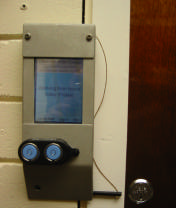
\includegraphics[width=0.5\textwidth]{./img/hermes_display.png}
  \caption{Das erste Hermes Display\cite{cheverest:2003:paper}}
  \label{img:hermesDisplay}
\end{figure}
Der Server wurde mit Java-Servlets realisiert und generiert HTML Webseiten, die auf den Displays angezeigt werden. Er bietet eine zentrale Datenbank für alle Daten des Systems und dient als Kommunikationseinheit mit einem SMS Gateway.
Eines der Hauptblickpunkte von Hermes war, dass das System leicht einsetzbar ist. Deswegen fiel die Entscheidung zur Wahl der Geräte auf PDAs. Zu der Zeit, als das Paper entstand waren PDAs die beste Wahl für kleine, handliche Geräte, welche per WLAN mit einem Server kommunizieren können. Zudem mussten die Geräte mit der Umweltpolitik der Universität übereinstimmen und sollten daher nicht viel Energie verbrauchen.
Um die Geräte vor Diebstahl zu schützen wurden Aluminiumhüllen für die PDAs entworfen, welche neben den Büroeingängen an die Wand geschraubt werden konnten und zudem auch als Diebstahlsicherung dienten. Um ungewünschte Interaktion zu verhindern wurden die Hülle so konzipiert, dass die Tasten nicht direkt zugänglich waren.\\

Die Funktionen von Hermes wurden in zwei Perspektiven aufgeteilt: Die Besitzerperspektive und die Besucherperspektive.
\subsubsection{Besitzerperspektive}
\textquote{Diese Perspektive ermöglicht dem Besitzer des Displays Nachrichten oder Bilder zu erstellen, die dann direkt auf dem PDA angezeigt werden oder Nachrichten zu lesen, die von Gästen für ihn hinterlassen wurden}\cite{cheverest:2003:paper}. Zudem kann der Nutzer animierte Gifs hochladen.
Der Nutzer kann die Perspektive von einem PC oder direkt am Display aufrufen, was ihm ermöglicht schnell beim Verlassen des Büros eine Nachricht zu schreiben. Um sich zu authentisieren muss er entweder seinen Nutzernamen und sein Passwort eingeben oder sich mit seinem iButton\footnote{Ein iButton ist ein Mikrochip in einer Metallhülle und dient beispielsweise zum Authentisieren des Besitzers \cite{iButton:website}} anmelden.
\subsubsection{Besucherperspektive}
\textquote{Besucher müssen sich vor dem PDA befinden, um mit dem System interagieren zu können}\cite{cheverest:2003:paper}. Sie können dem Besitzer des Raumes Nachrichten schreiben. Andere Besucher können jedoch nur die Nachricht sehen, die der Besitzer des Raumes eingestellt hat. Die Nachrichten von anderen Besucher kann nur der Besitzer einsehen, wodurch ein Vorteil im Bereich der Privatsphäre gegenüber Post-It Zetteln erzielt wurde.
\\
\\
Um das System zu testen haben die Entwickler eine Langzeitstudie über 15 Monate durchgeführt. Dabei haben sie im Vorfeld Bedenken geäußert, dass \textquote{die Nutzer Zeit brauchen bis sie neue Technologien in ihre tägliche Routine eingliedern}\cite{cheverest:2003:paper}.
Eines der enttäuschensten Ergebnisse war, dass es Nutzer gab, die trotz aufgehangenem Hermes Display weiterhin Post-Its an die Türen gehangen haben\cite{cheverest:2003:paper}.
Ein Ergebnis der Studie war, dass die Nutzer erst Vertrauen aufbauen müssen. \textquote{Nutzer nutzen ein neues System erst, wenn sie wissen, dass es funktioniert}\cite{cheverest:2003:paper}. Durch Verbindungsprobleme über das WLAN kam es dazu, dass das System ab und an nicht reagierte, wodurch es für die Nutzer schien, das Gerät wäre abgestürzt. Um dies zu beheben wurde das Metallgehäuse an der Stelle des WLAN Adapters geöffnet, damit das Gehäuse das Signal nicht weiter abschwächen konnte.
Es kam auch vor, dass Besucher vergaßen ihre Nachricht abzuschicken, wodurch deren Nachricht nicht mehr privat war und andere Nutzer sie sehen konnten. Das ermöglichte anderen Nutzern die Nachricht zu verändern oder sie zu missbrauchen um unangebrachte Nachrichten zu schreiben. Wenn der eigentliche Benutzer sich zudem auch authentisiert hat wurde die Nachricht dann in seinem Namen geschickt\cite{cheverest:2003:article}.
Manche Nutzer fanden es frustrierend nachdem sie eine temporäre Mitteilung eingestellt hatten eine alte Nachricht wiederherzustellen, da sie wieder durch den Prozess einer neuen Mitteilung gehen mussten. Als Lösung dafür wurde eine Möglichkeit eingebaut, mit der die Nutzer eine Standardnachricht einstellen konnten, die nach entfernen der temporären Nachricht wieder angezeigt wurde\cite{cheverest:2003:article}.
\\
\begin{figure}[h!]
  \centering
  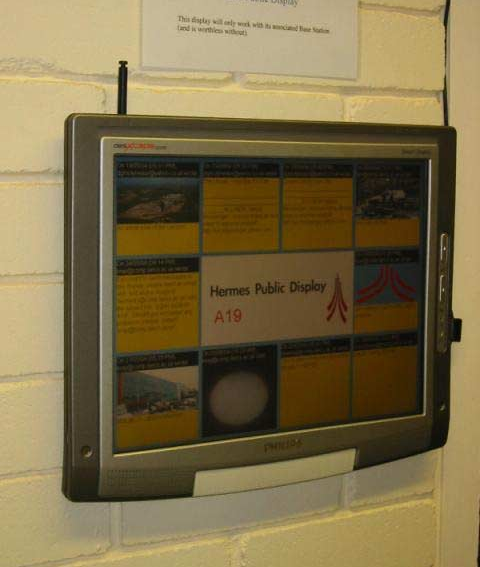
\includegraphics[width=0.5\textwidth]{./img/hermes_photoDisplay_short.png}
  \caption{Das erste Hermes Foto-Display\cite{cheverest:2012}}
  \label{img:hermesPhotoDisplay}
\end{figure}
\\
Um das Hermes System zu erweitern wurde später ein Foto-Display (Abb. \ref{img:hermesPhotoDisplay}) entwickelt\cite{cheveres:2005:hermes-bluetooth}. Da die Hermes-Displays sehr klein waren wurde dieses Display ausschließlich für Bilder verwendet.
Mit dieser Erweiterung war es den Nutzern möglich Bilder per MMS oder Bluetooth an das Gerät zu schicken oder mit der vorhandenen Displaykamera ein Bild zu schießen.
\\

\section{NetBoards}
NetBoards\cite{wood:2014}\cite{netboards:website} ist ein weiteres interessantes Projekt im Bereich interaktiver digitaler Türschilder. Es wurde 2014 an der Universität von Camebridge entwickelt und zielte darauf hin \textquote{die bereits vorhandenen Whiteboards und Pinnwände neben den Universitätsbüros mit großen, Touch-fähigen Bildschirmen zu erweitern oder zu ersetzen}\cite{wood:2014}.\\
Im Vergleich zum Hermes System, welches schon im Jahr 2003 veröffentlicht wurde, hatte sich einiges bezüglich Hardware geändert. \textquote{Displays sind billiger, größer, hochauflösender und energieeffizienter geworden}\cite{wood:2014}.
Dadurch konnten für NetBoards größere Bildschirme mit höherer Auflösung (Abb. \ref{img:netBoardsDisplay}) verwendet werden als beim Hermes System.
\begin{figure}[h!]
  \centering
    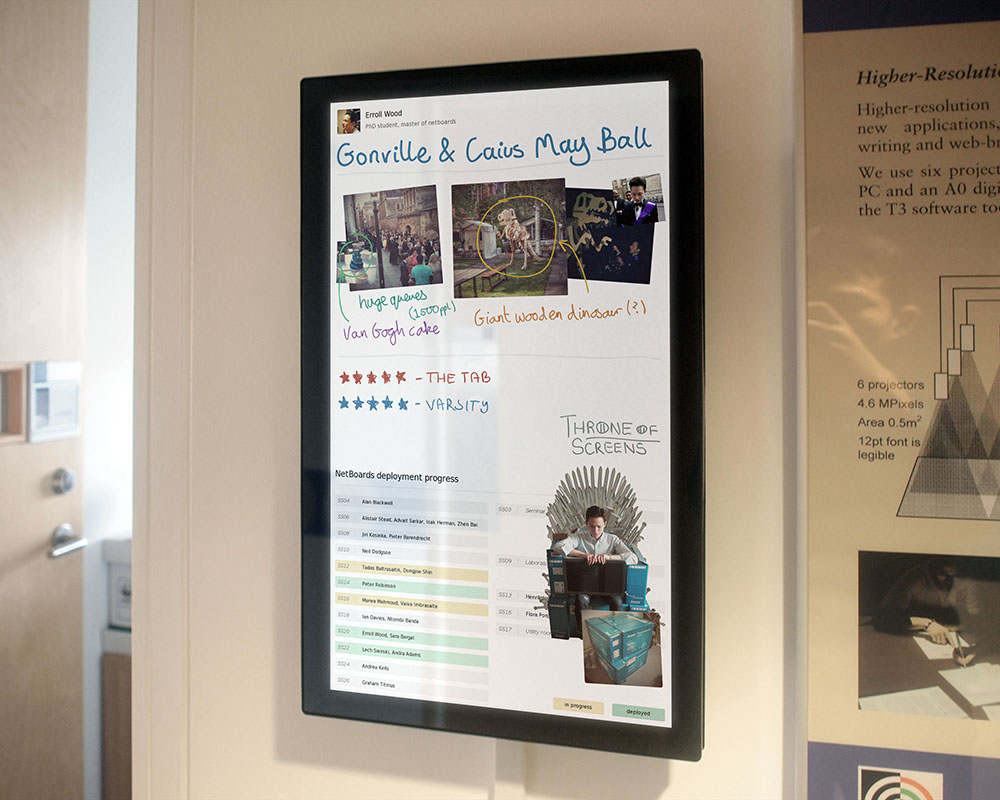
\includegraphics[width=0.7\textwidth]{./img/netBoards_display.png}
  \caption{Das NetBoards Display\cite{wood:2014}}
  \label{img:netBoardsDisplay}
\end{figure}
\\
% Prototyp Entwicklung
Die ersten Prototypen des NetBoard Systems bestanden jeweils aus einem 22 Zoll großem Touchscreen Monitor, der von einem Raspberry Pi\footnote{Ein Raspberry Pi ist ein kompakter Einplatinencomputer \cite{raspberrypi:website}} betrieben wurde.
Im ersten Experiment der Entwickler wurden fünf Prototypen verwendet um herauszufinden, ob die Boards akzeptiert werden und um typische Nutzerverhalten zu bestimmen.
\textquote{Diese wurden vor den Büros von Doktoranden, Post-Doktoranden und eines Professors aufgehangen um herauszufinden, wie diese unterschiedlichen Mitarbeiter mit dem System umgehen würden}\cite{wood:2014}
\textquote{Die Probanden konnten bei diesem Experiment Skizzen und Nachrichten zeichnen und Bilder per Web-Interface hochladen}\cite{wood:2014}. Zudem war es möglich Webseiten zu laden, die dann in einer Hintergrundschicht angezeigt werden konnten.
\\
Während des Experiments fanden die Entwickler heraus, dass die Boards schnell Aufmerksamkeit erzeugten. \textquote{Vorbeigehende Leute begannen spontan mit den Bildschirmen zu interagieren oder sogar die Besitzer direkt auf die Boards anzusprechen}\cite{wood:2014}.
Als Ergebnis des Experiments fanden die Entwickler heraus, dass 2 wichtige Faktoren die Akzeptanz der Nutzer gegenüber den Boards beeinflussen:
%Dependability
%Ease of use
\begin{itemize}
  \item \textbf{Zuverlässigkeit}: \textquote{Nutzer werden ein System nur benutzen wenn sie denken es funktioniert}\cite{wood:2014}
  \item \textbf{Benutzerfreundlichkeit}: \textquote{Angewöhnung der Nutzer an das System ist unwahrscheinlich, wenn das System schwer zu benutzen ist oder zu viel lernen erfordert}\cite{wood:2014}
\end{itemize}
Dadurch, dass für die Prototypen Touchscreens mit SAW-Technologie\footnote{Surface-Accoustic-Wave (dt.: Akkustische Oberflächenwelle) ist eine Technik um die Position von Fingern auf Displays zu ermitteln.} eingesetzt wurden war die Interaktion mit den Boards sehr ungenau, wodurch die Benutzerfreundlichkeit stark beeinträchtigt wurde.
% Raspberry Pi - zu schwach -> nutzung eines leistungsfähigerem rechners

%Das System bestand auch aus einem 22 Zoll großem Touchscreen, der im Hochformat an die Wand neben einem Büro geschraubt werden konnte. 
%\\
%\\
% System Spezifikationen
% Wie war die Testumgebung bei Wood?
% Irgendwelche Klassifizierungen? Views
% Wood Studie? - alles dazu - Ergebnisse
% Erweiterungen
%Benutzer hatten die Möglichkeit Nachrichten zu schreiben, Skizzen zu zeichnen oder Bilder anzeigen zu lassen.\cite{wood:2014}.



%Besitzer sowie Besucher konnten den Inhalt, der auf dem Display angezeigt wurde ändern, wodurch jedem Benutzer direkt in den präsentierten Inhalt eingreifen konnte. (Eben genau so wie ein öffentliches Whiteboard, wo jeder der vorbei geht etwas ändern kann)  -- hier könnte ich vllt auch das beispiel der mensa whiteboards bringen ---- Kinderhacksteak anstelle vom Rinderhacksteak


% - Netboards by Errol Wood, Peter Robinson
%   * neues Projekt (2014)
%   * basierend auf Whiteboards
%   * für große, mit dem Netzwerk verbundene, touch Displays % cite wood Netboards
%   * Nutzer können Nachrichten, Sketches, Bilder auf dem Board schreiben
%   * Problem: jeder kann auf Board schreiben --> abusing (hab ich sehr stark gemerkt)
%   * Drei Frontend Layer
%     # UI Elements (Sidebar,Büronutzer infos)
%     # Content Layer
%     # Webpage backround layer
%   * PaperJS als Editor Grundlage
%   * Drag & Drop Bilder vom PC aufs Board
%   * Set Status

\section{Andere}
McCarthy: OutCast\cite{mccarthy:2001}
% - Andere Displays außerhalb von Büros:
%   * Dynamic Door Displays by Nguyen et al
%   * OutCast by McCarthy et al
% 
% - Zusätlich gibt es auch noch ein Forschungsfeld für Displays am Arbeitsplatz
% 
% - Andere Zusammenhängende Arbeiten:
%   * Semi-Public-Displays for Small, Co-located Groups by Elaine M. Huang, Elizabeth D. Mynatt
%   * UniCast, OutCast & GroupCast: Three Steps Toward Ubiquitous, Peripheral Displays
%   * ben Schneiderman 2002 Leonardos Laptop 